\section{ERP Task Engine Layer}
% Provides the core task engine for document processing. It is responsible for triggering agents, managing task queues, and orchestrating the flow of tasks. \\
% \hline

% Dividing the first table into multiple frames with 3 rows each

\begin{frame}
    \frametitle{ERP Task Engine Layer - Components}
    \begin{figure}
        \centering
        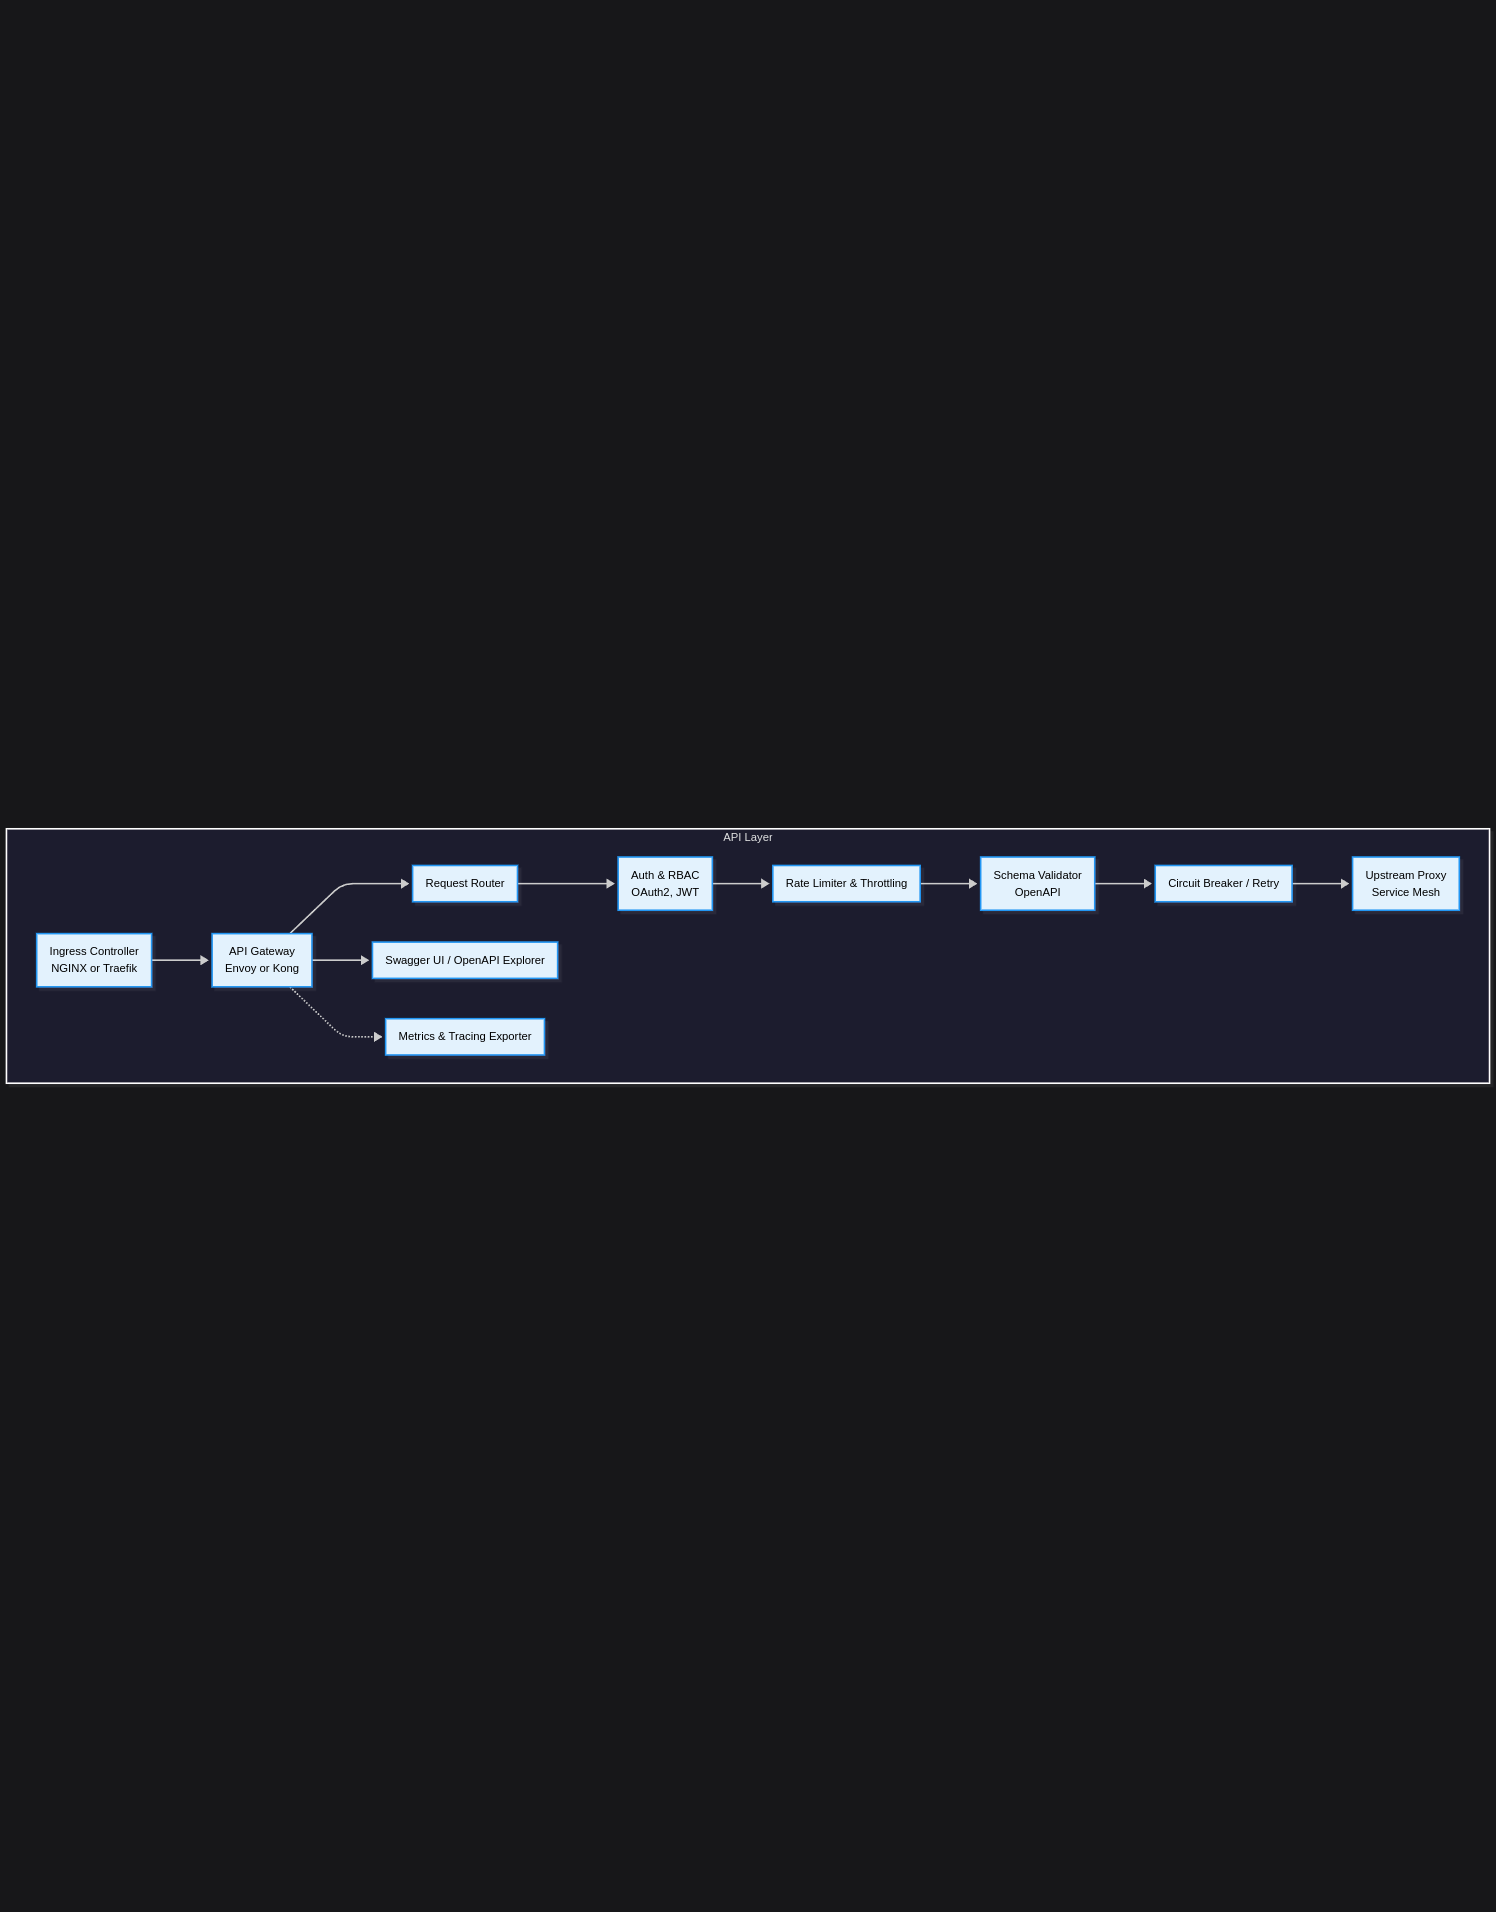
\includegraphics[width=0.3\textwidth]{erp/layout.png} % Adjusted the scale of the image to 0.5
        \caption{ERP Task Engine Layer Overview}
    \end{figure}
\end{frame}

\begin{frame}
    \frametitle{ERP Task Engine Layer - Sequence Flow}
    \begin{figure}
        \centering
        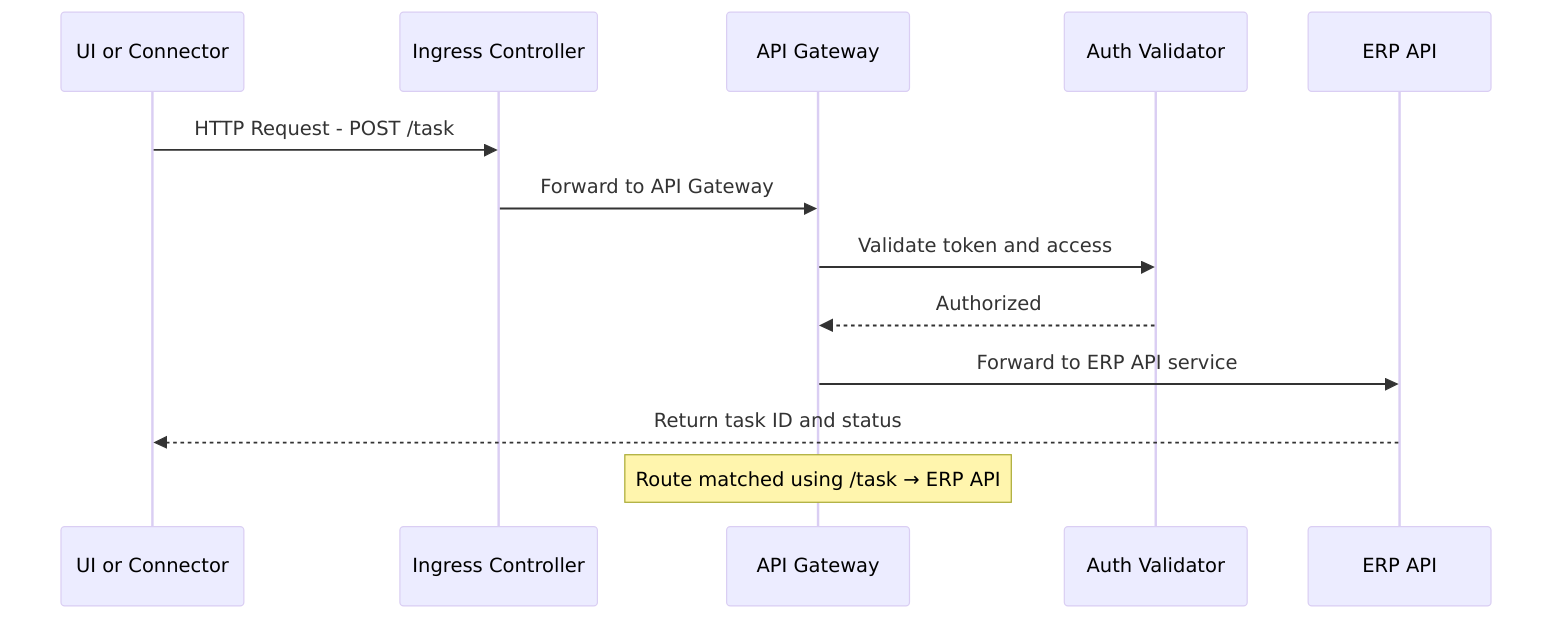
\includegraphics[width=0.8\textwidth]{erp/sequence.pdf} % Adjusted the scale of the image to 0.5
        \caption{ERP Task Engine Layer Workflow}
    \end{figure}
\end{frame}


\begin{frame}
    \frametitle{ERP Task Engine Layer }
    \begin{itemize}
        \item \textbf{Task Manager}: Create, update, and assign tasks linked to documents and agents.
        \item \textbf{Workflow Controller}: Control state transitions, enforce review rules.
        \item \textbf{Review Interface}: Collect reviewer decisions and confirmations.
        \item \textbf{Project Planner}: Organize project timeline, deliverables, dependencies.
        \item \textbf{Task Tracker}: Track progress, task time, SLA milestones.
        \item \textbf{Notification System}: Send alerts, reminders, escalation messages.
    \end{itemize}
\end{frame}



\begin{frame}
    \frametitle{ERP Task Engine Layer }
    \begin{itemize}
        \item \textbf{Revision Alert Engine}: Trigger dependent task revision when spec changes are detected.
        \item \textbf{Project Query Agent}: Provide real-time status and updates by interacting with multiple project agents.
        \item \textbf{Analytics Engine}: Report task durations, agent success rate, delays.
        \item \textbf{File Browser}: View, search, and link documents to tasks.
        \item \textbf{ERP API Interface}: Accept and respond to API calls from UI and other layers.
        \item \textbf{Task Database}: Store all task metadata, decisions, timestamps, and links.
    \end{itemize}
\end{frame}


% % Dividing the second table into multiple frames with 3 rows each
% \begin{frame}
%     \frametitle{Technical Responsibilities - Part 1}
%     \begin{table}[h!]
% \centering
% \renewcommand{\arraystretch}{1.2}
% \begin{tabular}{|p{3cm}|p{7cm}|}
% \hline
% \textbf{Component} & \textbf{Technical Responsibility} \\
% \hline
% Task Manager & Exposes REST services to create, update, fetch, and assign tasks \\
% \hline
% Workflow Controller & Implements task FSM logic with configurable state transitions \\
% \hline
% Review Interface & Frontend and backend views integrated with task models \\
% \hline
% \end{tabular}
% \caption{ERP Task Engine - Technical Responsibilities (Part 1)}
% \end{table}
% \end{frame}

% \begin{frame}
%     \frametitle{Technical Responsibilities - Part 2}
%     \begin{table}[h!]
% \centering
% \renewcommand{\arraystretch}{1.2}
% \begin{tabular}{|p{3cm}|p{7cm}|}
% \hline
% \textbf{Component} & \textbf{Technical Responsibility} \\
% \hline
% Project Planner & Gantt and dependency logic using temporal fields and project graph \\
% \hline
% Task Tracker & Tracks task durations and stages via DB triggers or polling \\
% \hline
% Notification System & Hooks into Prometheus Alertmanager or custom notifier for emails, Slack, SMS \\
% \hline
% \end{tabular}
% \caption{ERP Task Engine - Technical Responsibilities (Part 2)}
% \end{table}
% \end{frame}

% \begin{frame}
%     \frametitle{Technical Responsibilities - Part 3}
%     \begin{table}[h!]
% \centering
% \renewcommand{\arraystretch}{1.2}
% \begin{tabular}{|p{3cm}|p{7cm}|}
% \hline
% \textbf{Component} & \textbf{Technical Responsibility} \\
% \hline
% Revision Alert Engine & Listens to changes in spec docs, triggers downstream task regeneration \\
% \hline
% Project Query Agent & Uses vector or indexed metadata to answer queries via LLM or keyword logic \\
% \hline
% Analytics Engine & Uses TimescaleDB or dashboard backend to show task KPIs \\
% \hline
% \end{tabular}
% \caption{ERP Task Engine - Technical Responsibilities (Part 3)}
% \end{table}
% \end{frame}

% \begin{frame}
%     \frametitle{Technical Responsibilities - Part 4}
%     \begin{table}[h!]
% \centering
% \renewcommand{\arraystretch}{1.2}
% \begin{tabular}{|p{3cm}|p{7cm}|}
% \hline
% \textbf{Component} & \textbf{Technical Responsibility} \\
% \hline
% File Browser & Embedded S3/MinIO explorer with task linkage metadata \\
% \hline
% ERP API Interface & REST/GraphQL endpoints with role-based access control \\
% \hline
% Task Database & Postgres with schema for task, versions, relations, timestamps \\
% \hline
% \end{tabular}
% \caption{ERP Task Engine - Technical Responsibilities (Part 4)}
% \end{table}
% \end{frame}

